\section{Applications to Curves}

\noindent
\boxit{One-Parameter Families of Curves}

\noindent
We begin with two examples of families of curves generated by varying
a parameter over a set of real numbers.

\begin{example}\label{example:4.5.1} \rm
For each value of the parameter $c$, the equation
\begin{equation} \label{eq:4.5.1}
y-cx^2=0
\end{equation}
defines a curve in the $xy$-plane. If $c \ne0$, the curve is a
parabola through the origin, opening upward if $c>0$ or downward if
$c<0$.   If $c=0$, the curve is the $x$ axis (Figure~\ref{figure:4.5.1}).
\end{example}

\begin{figure}[H]
  \centering
  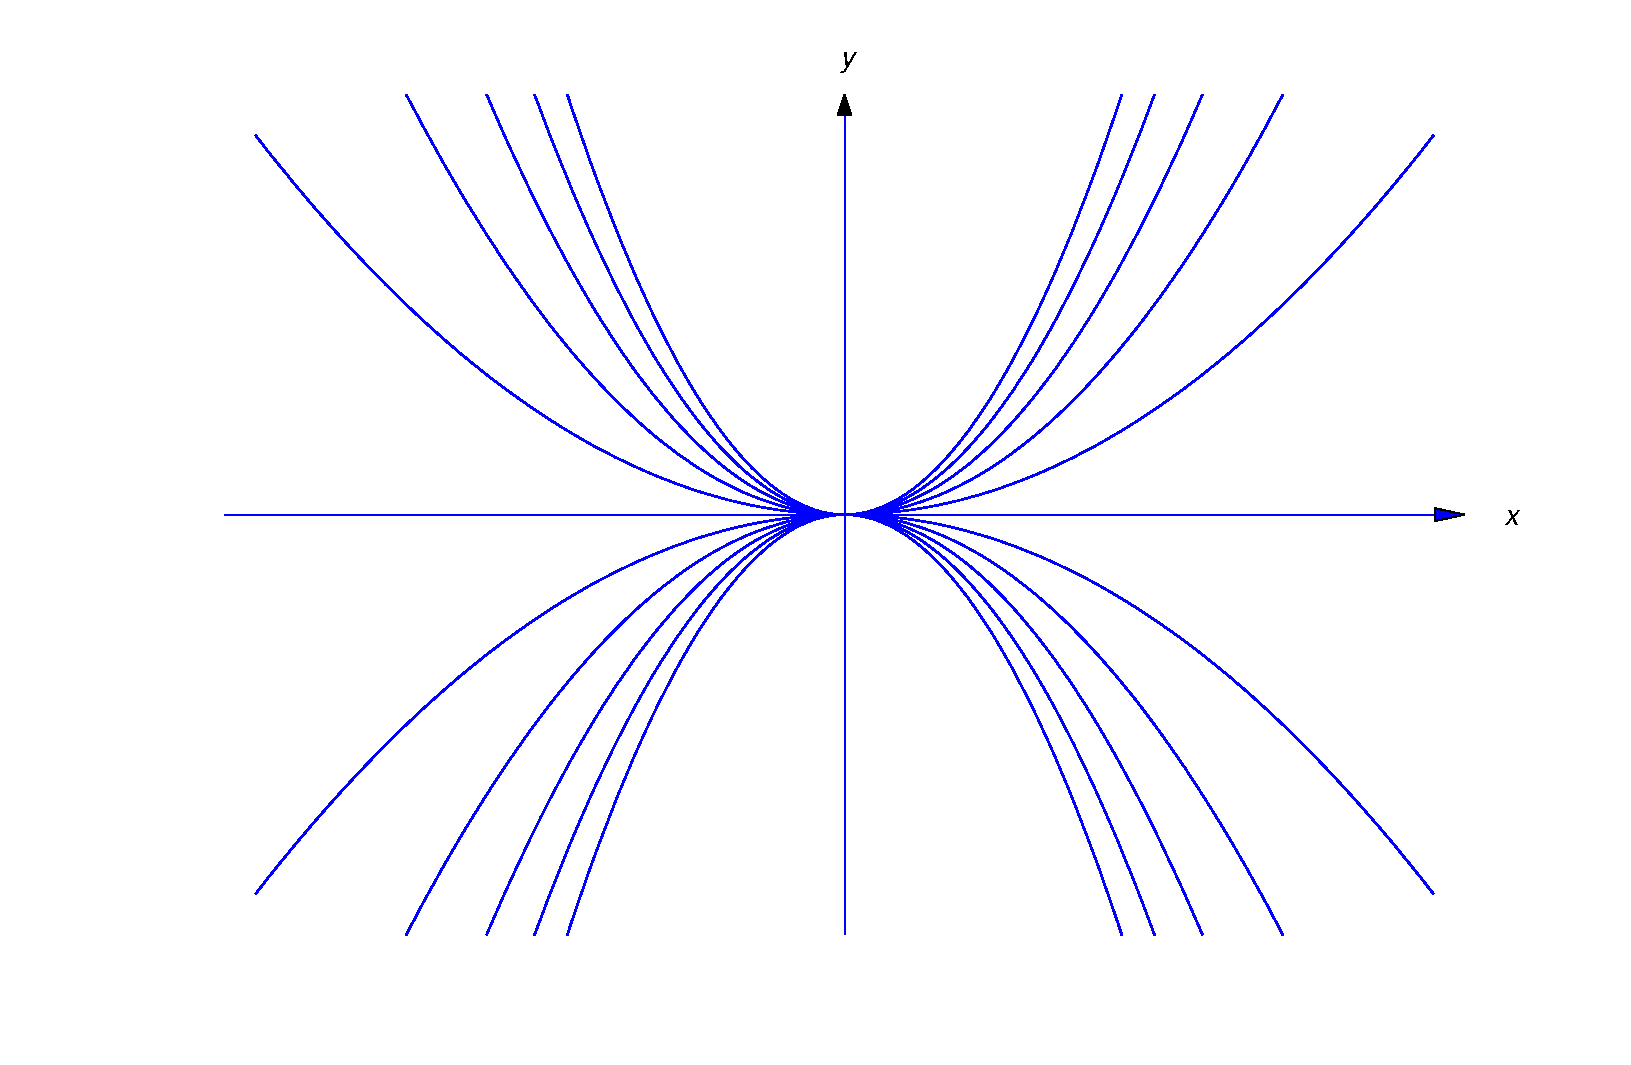
\includegraphics[bb=-78 148 689 643,width=5.67in,height=3.66in,keepaspectratio]{fig040501}
\color{blue}
  \caption{ A family of curves defined by $y-cx^2=0$}
  \label{figure:4.5.1}
\end{figure}

\begin{example} \label{example:4.5.2} \rm
For each value of the parameter $c$ the equation
\begin{equation} \label{eq:4.5.2}
y=x+c
\end{equation}
 defines a line with slope 1(Figure~\ref{figure:4.5.2}).
\end{example}

\begin{figure}[htbp]
\color{blue}
  \begin{minipage}[b]{0.5\linewidth}
    \centering
   \scalebox{.65}{
  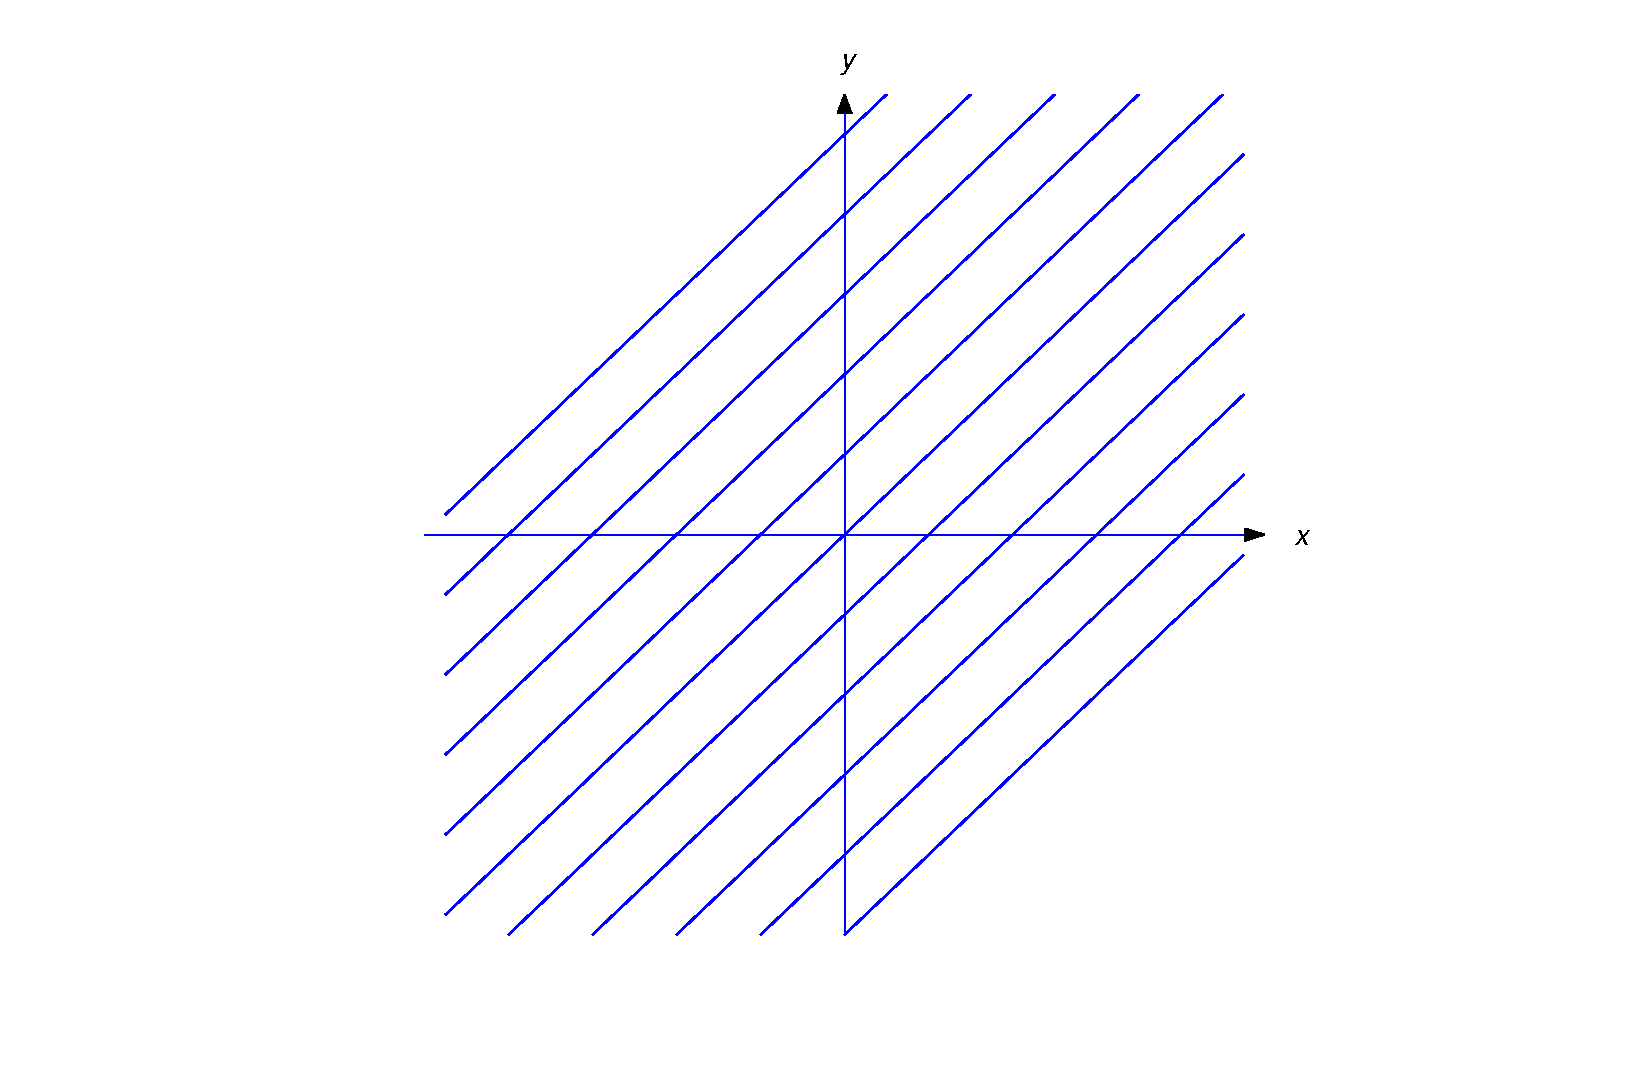
\includegraphics[bb=-78 148 689 643,width=5.67in,height=3.66in,keepaspectratio]{fig040502}}
  \caption{ A family of lines defined by $y=x+c$}
  \label{figure:4.5.2}
  \end{minipage}
  \hspace{0.6cm}
  \begin{minipage}[b]{0.5\linewidth}
    \centering
   \scalebox{.65}{
  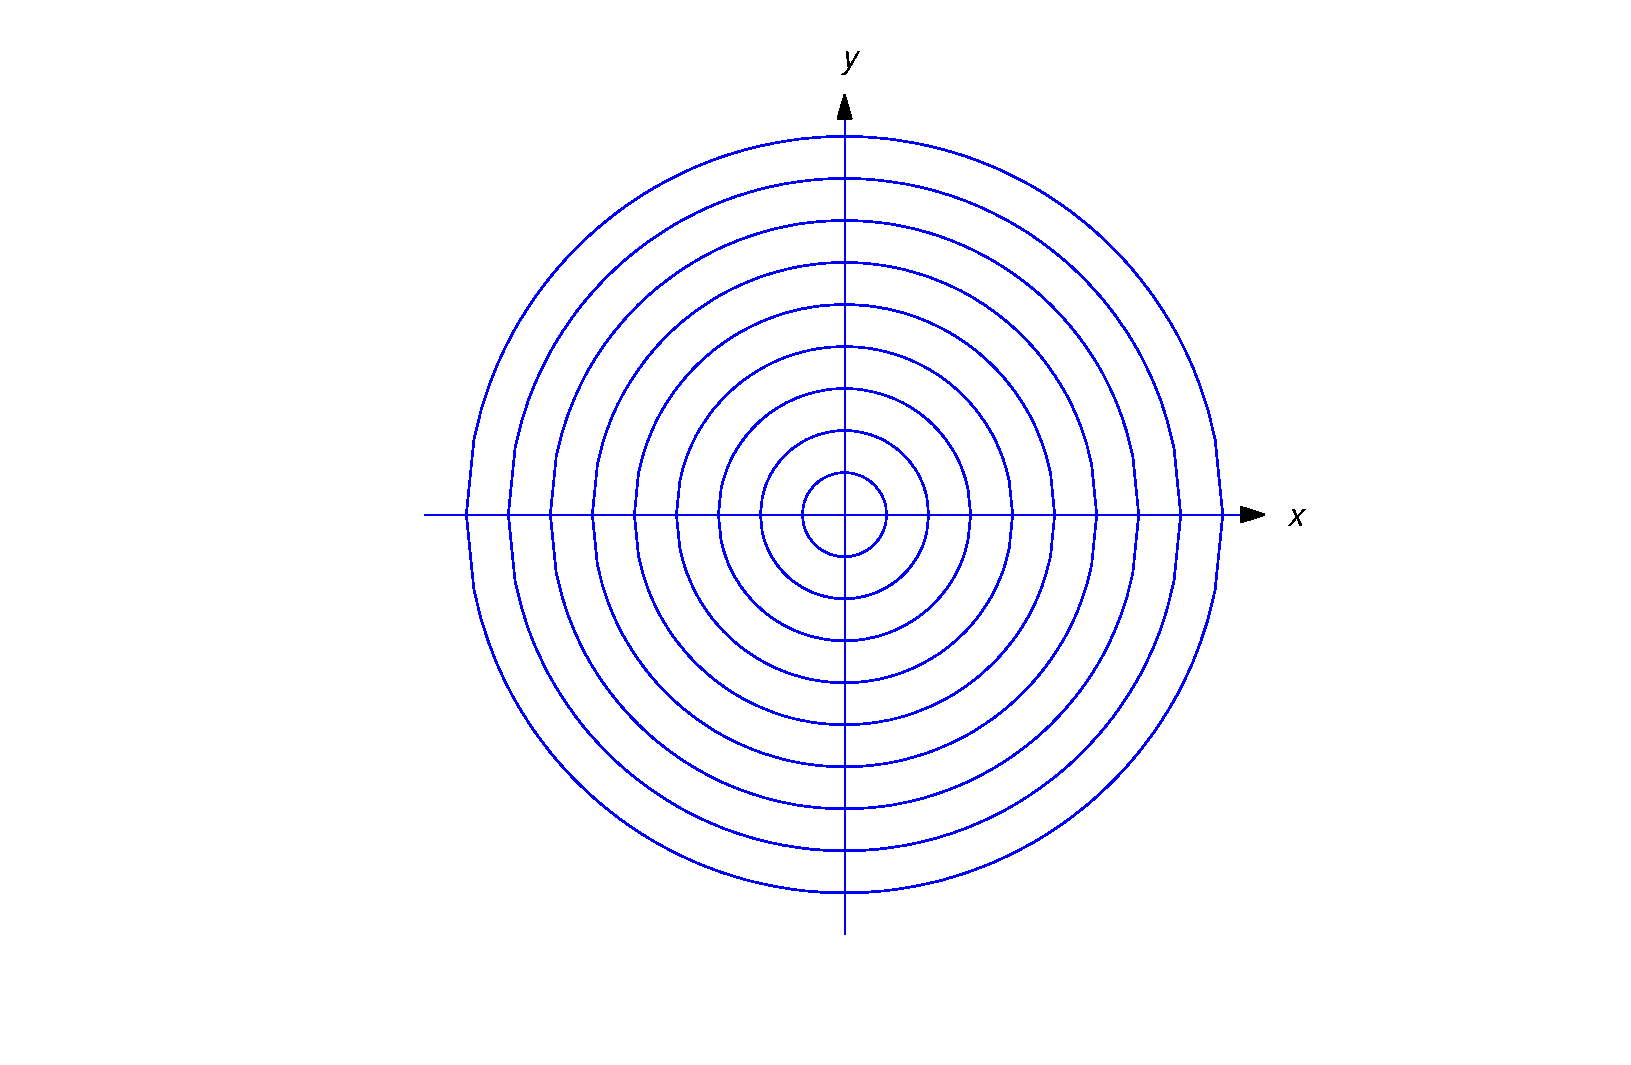
\includegraphics[bb=-78 148 689 643,width=5.67in,height=3.66in,keepaspectratio]{fig040503}}
  \caption{ A family of circles defined by $x^2+y^2-c^{2}=0$}
  \label{figure:4.5.3}
  \end{minipage}
\end{figure}

\begin{definition}\color{blue} \label{thmtype:4.5.1}
\rm An equation that can be written in the form
 \begin{equation} \label{eq:4.5.3}
H(x,y,c)=0
\end{equation}
is said to define a {\color{blue}\it one-parameter family of curves\/} if, for
each value of $c$ in some nonempty set of real numbers, the set of
points $(x,y)$ that satisfy  \eqref{eq:4.5.3} forms a curve in the
$xy$-plane.
\end{definition}

Equations \eqref{eq:4.5.1} and \eqref{eq:4.5.2} define one--parameter families
of curves. (Although \eqref{eq:4.5.2} isn't  in the form \eqref{eq:4.5.3}, it
can be written in this form as $y-x-c=0$.)

\begin{example}\label{example:4.5.3} \rm
If $c>0$,  the graph of the equation
\begin{equation} \label{eq:4.5.4}
x^2+y^2-c=0
\end{equation}
is a circle with center at $(0,0)$ and radius $\sqrt{c}$. If $c=0$, the
graph is the single point $(0,0)$. (We don't regard a single point as
a curve.) If $c<0$, the equation has no graph. Hence, \eqref{eq:4.5.4}
defines a one--parameter family of curves for positive values of $c$.
This family consists of all circles centered at $(0,0)$
(Figure~\ref{figure:4.5.3}).
\end{example}

\begin{example}\label{example:4.5.4} \rm
 The equation
$$
x^2+y^2+c^2=0
$$
does not define a one-parameter family of curves, since no $(x,y)$
satisfies the equation if $c\ne0$, and only the single point $(0,0)$
satisfies it if $c=0$. \bbox
\end{example}

Recall from Section~1.2 that the graph of a solution of a
differential equation is called an {\color{blue}\it integral curve\/} of the
equation. Solving a first order differential equation usually produces
a one--parameter family of integral curves of the equation. Here we
are interested in the converse problem:
given a one--parameter family of curves, is there a first order
differential equation for which every  member of the family is an integral
curve.
This suggests the next definition.

\begin{definition}\color{blue} \label{thmtype:4.5.2}
\rm If every curve in a one-parameter family defined by the equation
\begin{equation} \label{eq:4.5.5}
H(x,y,c)=0
\end{equation}
is an integral curve of the first order differential equation
\begin{equation} \label{eq:4.5.6}
F(x,y,y')=0,
\end{equation}
then  \eqref{eq:4.5.6} is said to be a {\color{blue}\it differential equation
for the family.\/}
\end{definition}

To find a differential equation for a one--parameter family we
differentiate its defining equation \eqref{eq:4.5.5} implicitly with
respect to $x$, to obtain
\begin{equation} \label{eq:4.5.7}
H_x(x,y,c)+H_y(x,y,c)y'=0.
\end{equation}
If this equation doesn't, then it's a differential
equation for the family. If it does contain $c$, it may be
possible to obtain a differential equation for the family by
eliminating $c$ between \eqref{eq:4.5.5} and \eqref{eq:4.5.7}.

\begin{example}\label{example:4.5.5}  \rm
Find a differential equation for the family of curves defined by
\begin{equation}  \label{eq:4.5.8}
y=cx^2.
\end{equation}
\end{example}

\solution Differentiating
\eqref{eq:4.5.8} with respect to $x$ yields
$$
y'=2cx.
$$
 Therefore $c=y'/2x$, and substituting this into
\eqref{eq:4.5.8} yields
$$
y={xy'\over2}
$$
 as a differential equation for the family of
curves defined by \eqref{eq:4.5.8}.  The graph of any function of
the form $y=cx^2$ is an integral curve of this equation. \bbox

The next example shows that members of a given family of curves
may be obtained by joining  integral curves for more than one
differential equation.

\begin{example}\label{example:4.5.6} \rm
\mbox{}
\begin{alist}
\item %(a)
Try to find a differential equation for the family of lines tangent
to the parabola $y=x^2$.

\item %(b)
Find two tangent lines to  the parabola $y=x^2$ that pass
through $(2,3)$, and find the points of tangency.
\end{alist}
\end{example}

\solutionpart{a} The equation of the line through a given point
$(x_0,y_0)$ with slope $m$ is
\begin{equation}  \label{eq:4.5.9}
y=y_0+m(x-x_0).
\end{equation}
If $(x_0,y_0)$ is on the parabola, then $y_0=x_0^2$ and the slope of
the tangent line through ($x_0,x_0^2)$ is $m=2x_0$; hence,
\eqref{eq:4.5.9} becomes
$$
y=x_0^2+2x_0(x-x_0),
$$
 or, equivalently,
\begin{equation} \label{eq:4.5.10}
y=-x_0^2+2x_0x.
\end{equation}
Here $x_0$ plays the role of the constant $c$ in
Definition~\ref{thmtype:4.5.1}; that is, varying $x_0$ over
$(-\infty,\infty)$ produces the family of tangent lines to the
parabola $y=x^2$.

Differentiating \eqref{eq:4.5.10} with respect to $x$ yields
$y'=2x_0$..
We can express $x_0$ in terms of $x$ and $y$ by rewriting
\eqref{eq:4.5.10} as
$$
x_0^2-2x_0x+y=0
$$
and using the quadratic formula to obtain
 \begin{equation}\label{eq:4.5.11}
 x_0=x\pm\sqrt{x^2-y}.
\end{equation}
We must choose the plus sign in \eqref{eq:4.5.11} if $x<x_0$
and the minus sign if $x>x_0$;   thus,
$$
x_0=\left(x+\sqrt{x^2-y}\right)\mbox{\, if \,} x<x_0
$$
 and
$$
x_0=\left(x-\sqrt{x^2-y}\right)\mbox{\, if \,} x>x_0.
$$
Since $y'=2x_0$, this implies that
\begin{equation} \label{eq:4.5.12}
y'=2\left(x+\sqrt{x^2-y}\right),\mbox{\quad if \quad} x<x_0
\end{equation}
 and
\begin{equation} \label{eq:4.5.13}
y'=2\left(x-\sqrt{x^2-y}\right),\mbox{\quad if \quad}x>x_0.
\end{equation}
Neither \eqref{eq:4.5.12} nor \eqref{eq:4.5.13} is a differential equation for
the family of tangent lines to the parabola $y=x^2$. However, if each
tangent line is regarded as consisting of two {\color{blue}\it tangent half
lines\/} joined at the point of tangency,   \eqref{eq:4.5.12} is a
differential equation for the family of tangent half lines on which
$x$ is less than the abscissa of the point of tangency
(Figure~\ref{figure:4.5.4}\part{a}), while \eqref{eq:4.5.13} is a
differential
equation for the family of tangent half lines on which $x$ is greater
than this abscissa (Figure~\ref{figure:4.5.4}(b)). The
parabola $y=x^2$ is also an integral curve of both \eqref{eq:4.5.12} and
\eqref{eq:4.5.13}.

\begin{figure}[H]
  \centering
  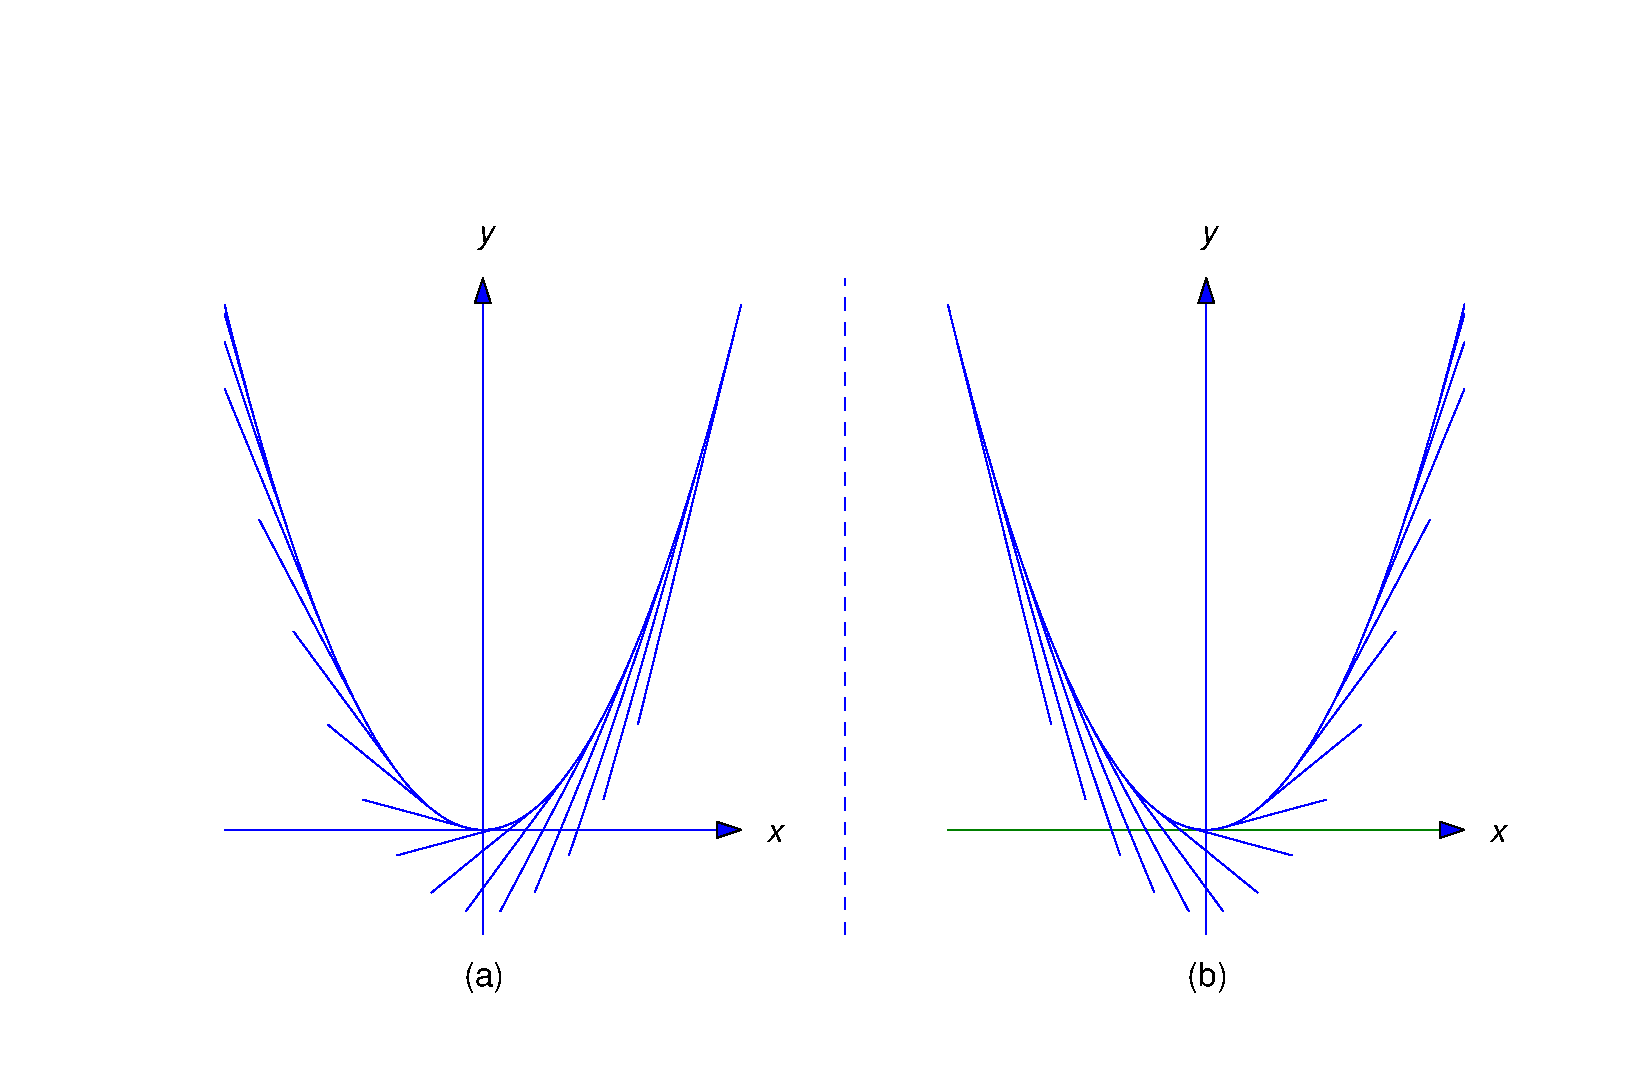
\includegraphics[bb=-78 148 689 643,width=5.67in,height=3.66in,keepaspectratio]{fig040504}
\color{blue}
  \caption{}
  \label{figure:4.5.4}
\end{figure}

\solutionpart{b}
From \eqref{eq:4.5.10} the point $(x,y)=(2,3)$ is on the tangent line
through $(x_0,x_0^2)$ if and only if
$$
3=-x_0^2+4x_0,
$$
which is equivalent to
$$
x_0^2-4x_0+3=(x_0-3)(x_0-1)=0.
$$
Letting $x_0=3$ in \eqref{eq:4.5.10} shows that $(2,3)$ is on the line
$$
y=-9+6x,
$$
which is tangent to the parabola at $(x_0,x_0^2)=(3,9)$, as shown in
Figure~\ref{figure:4.5.5}

Letting $x_0=1$ in \eqref{eq:4.5.10} shows that $(2,3)$ is on the line
$$
y=-1+2x,
$$
which is tangent to the parabola at $(x_0,x_0^2)=(1,1)$, as shown in
Figure~\ref{figure:4.5.5}.

 \vspace*{-15pt}
\begin{figure}[H]
  \centering
  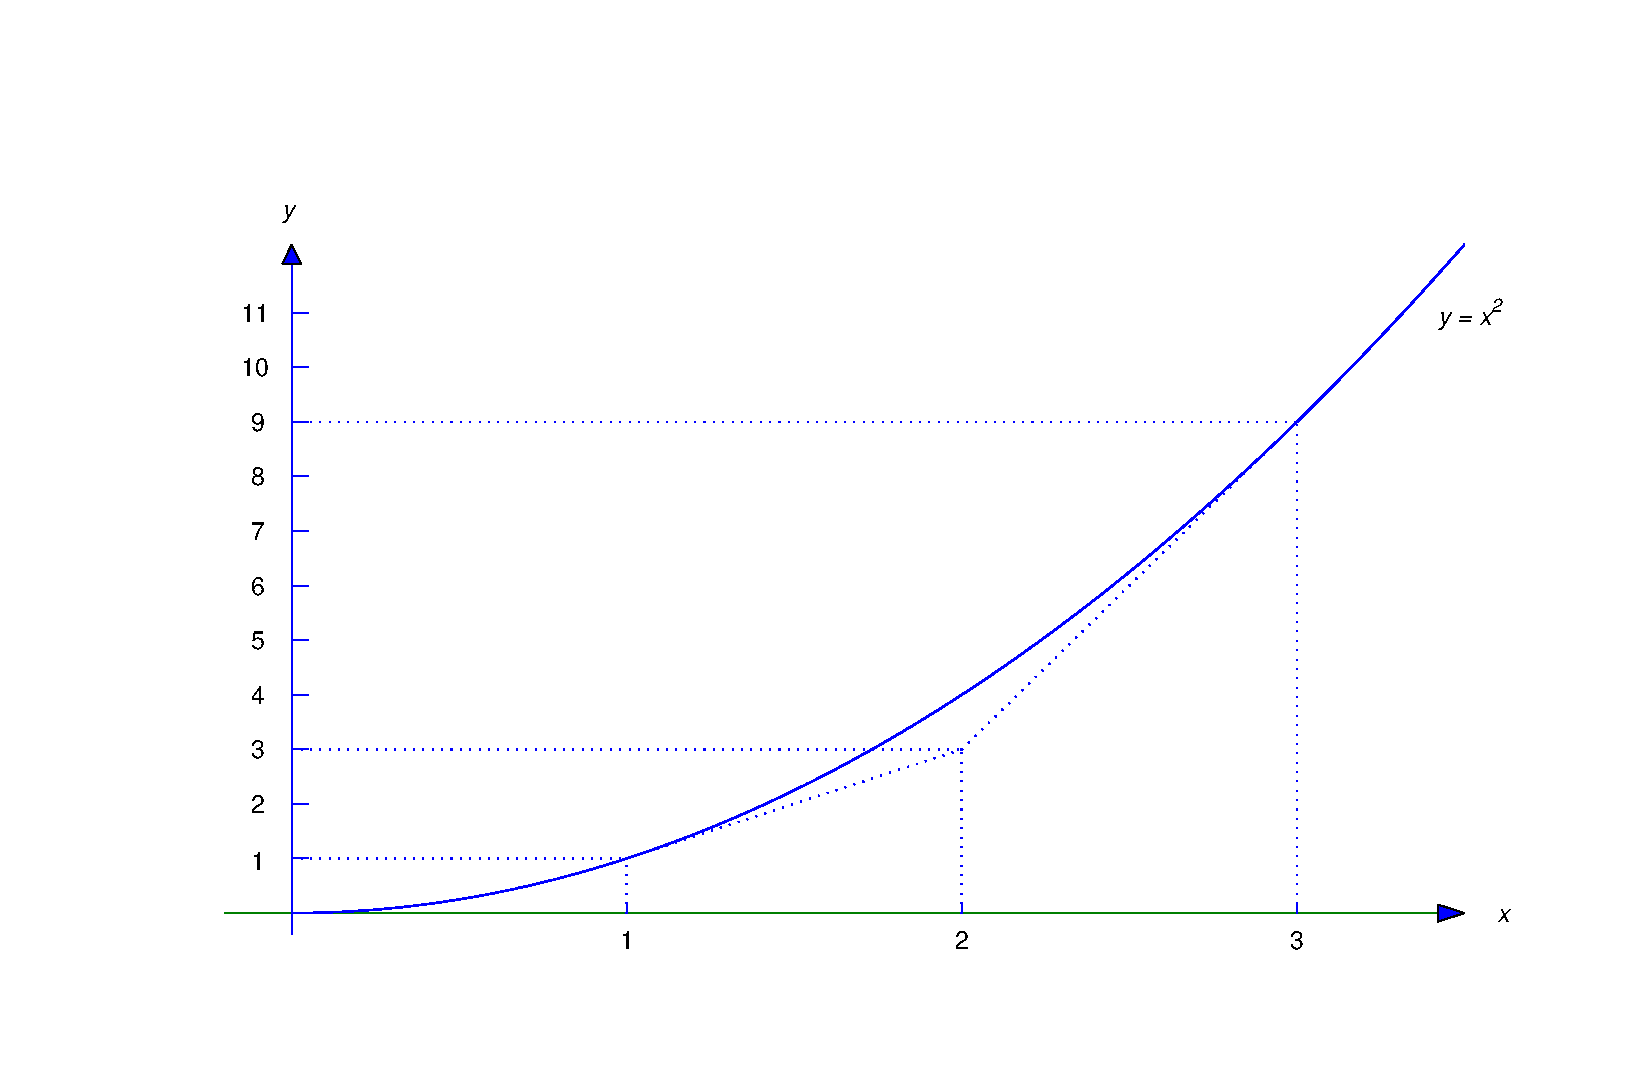
\includegraphics[bb=-78 148 689 643,width=5.67in,height=3.66in,keepaspectratio]{fig040505}
  \caption{}
  \label{figure:4.5.5}
\end{figure}

\boxit{Geometric Problems}

\noindent
We now consider some geometric problems that can be solved by means of
differential equations.

\begin{example}\label{example:4.5.7}   \rm
Find curves $y=y(x)$ such that every point $(x_0,y(x_0))$ on the curve
is the midpoint of the line segment with endpoints on the coordinate
axes and tangent to the curve at $(x_0,y(x_0))$
(Figure~\ref{figure:4.5.6}).
\end{example}

\solution
 The equation of the  line tangent to the curve at $P=(x_0,y(x_0)$ is
$$
y=y(x_0)+y'(x_0)(x-x_0).
$$
If we denote the $x$ and $y$ intercepts of the tangent line by $x_I$
and $y_I$ (Figure~\ref{figure:4.5.6}), then
\begin{equation} \label{eq:4.5.14}
0=y(x_0)+y'(x_0)(x_I-x_0)
\end{equation}
 and
\begin{equation} \label{eq:4.5.15}
y_I=y(x_0)-y'(x_0)x_0.
\end{equation}
From Figure~\ref{figure:4.5.6}, $P$ is the midpoint of the line segment
connecting $(x_I,0)$ and $(0,y_I)$ if and only if $x_I=2x_0$ and
$y_I=2y(x_0)$. Substituting the first of these conditions into
\eqref{eq:4.5.14} or the second into \eqref{eq:4.5.15} yields
$$
y(x_0)+y'(x_0)x_0=0.
$$
Since $x_0$ is arbitrary we drop the subscript and conclude that
$y=y(x)$  satisfies
$$
y+xy'=0,
$$
which can be rewritten as
$$
(xy)'=0.
$$
Integrating  yields $xy=c$,  or
$$
y={c\over x}.
$$
If $c=0$ this curve is the line $y=0$, which does not satisfy the
geometric requirements imposed by the problem;   thus, $c\ne0$, and the
solutions define a family of hyperbolas (Figure~\ref{figure:4.5.7}).

\begin{figure}[htbp]
\color{blue}
  \begin{minipage}[b]{0.5\linewidth}
    \centering
   \scalebox{.65}{
  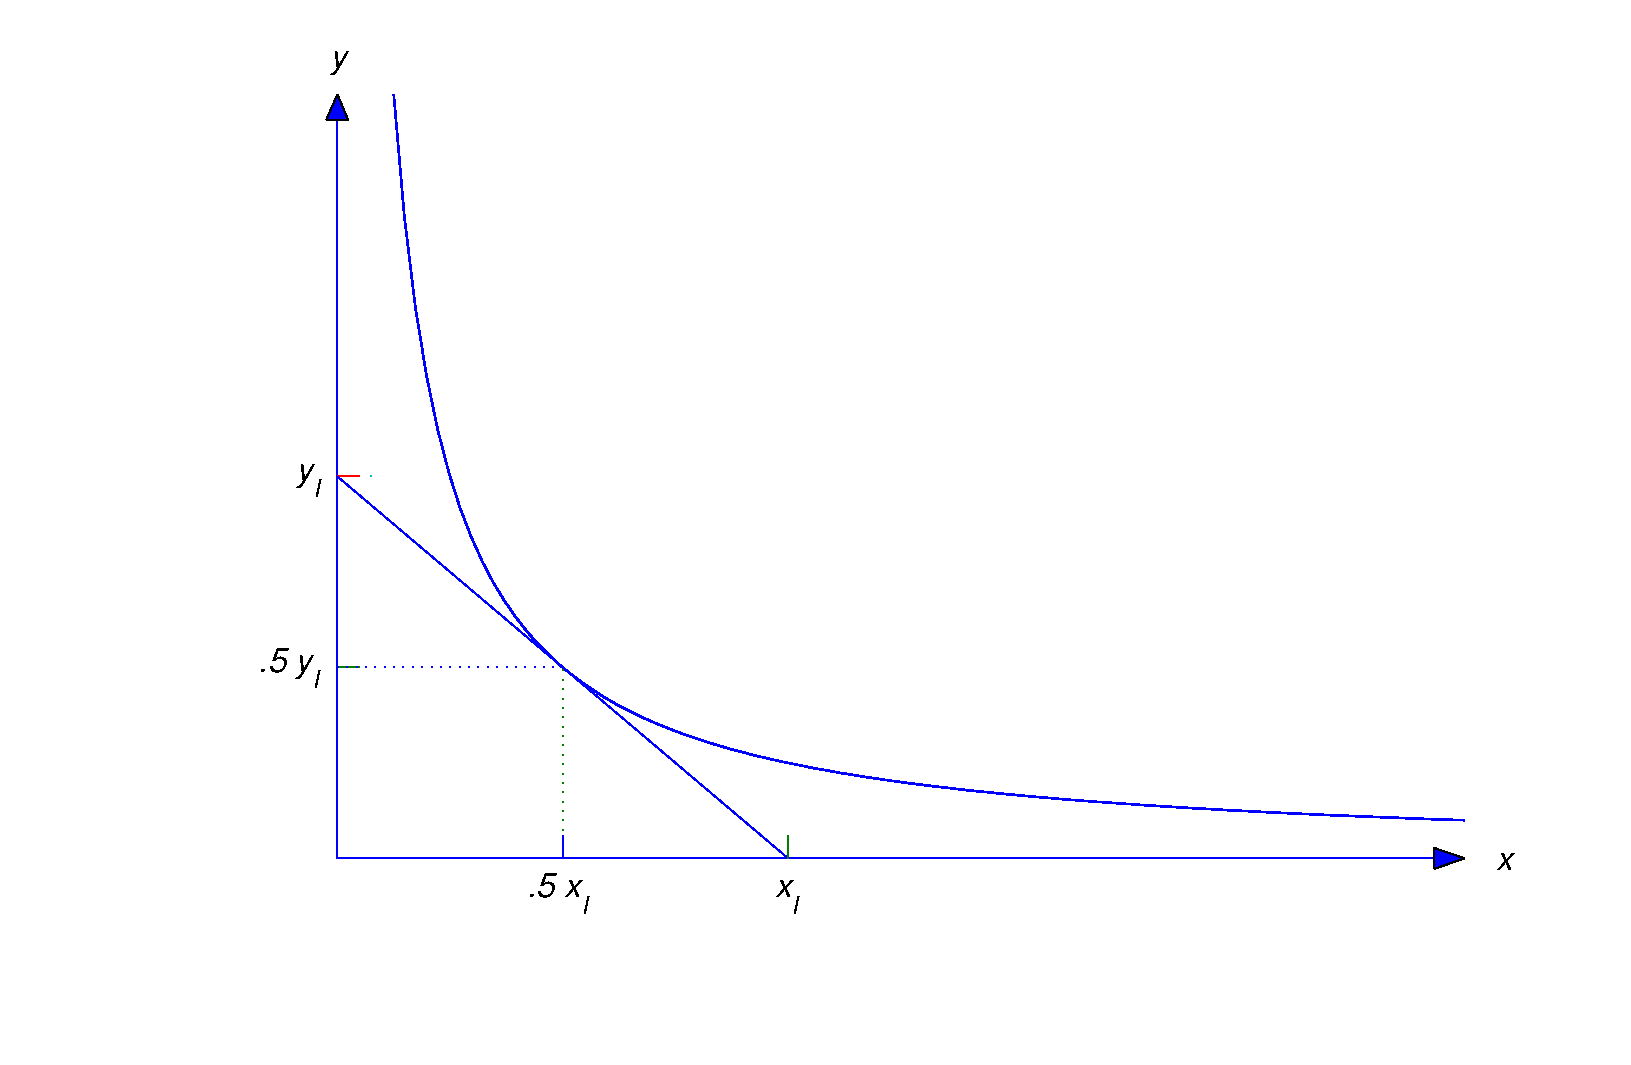
\includegraphics[bb=-78 148 689 643,width=5.67in,height=3.66in,keepaspectratio]{fig040506} }
\caption{}
  \label{figure:4.5.6}
  \end{minipage}
  \hspace{0.6cm}
  \begin{minipage}[b]{0.5\linewidth}
    \centering
   \scalebox{.65}{
  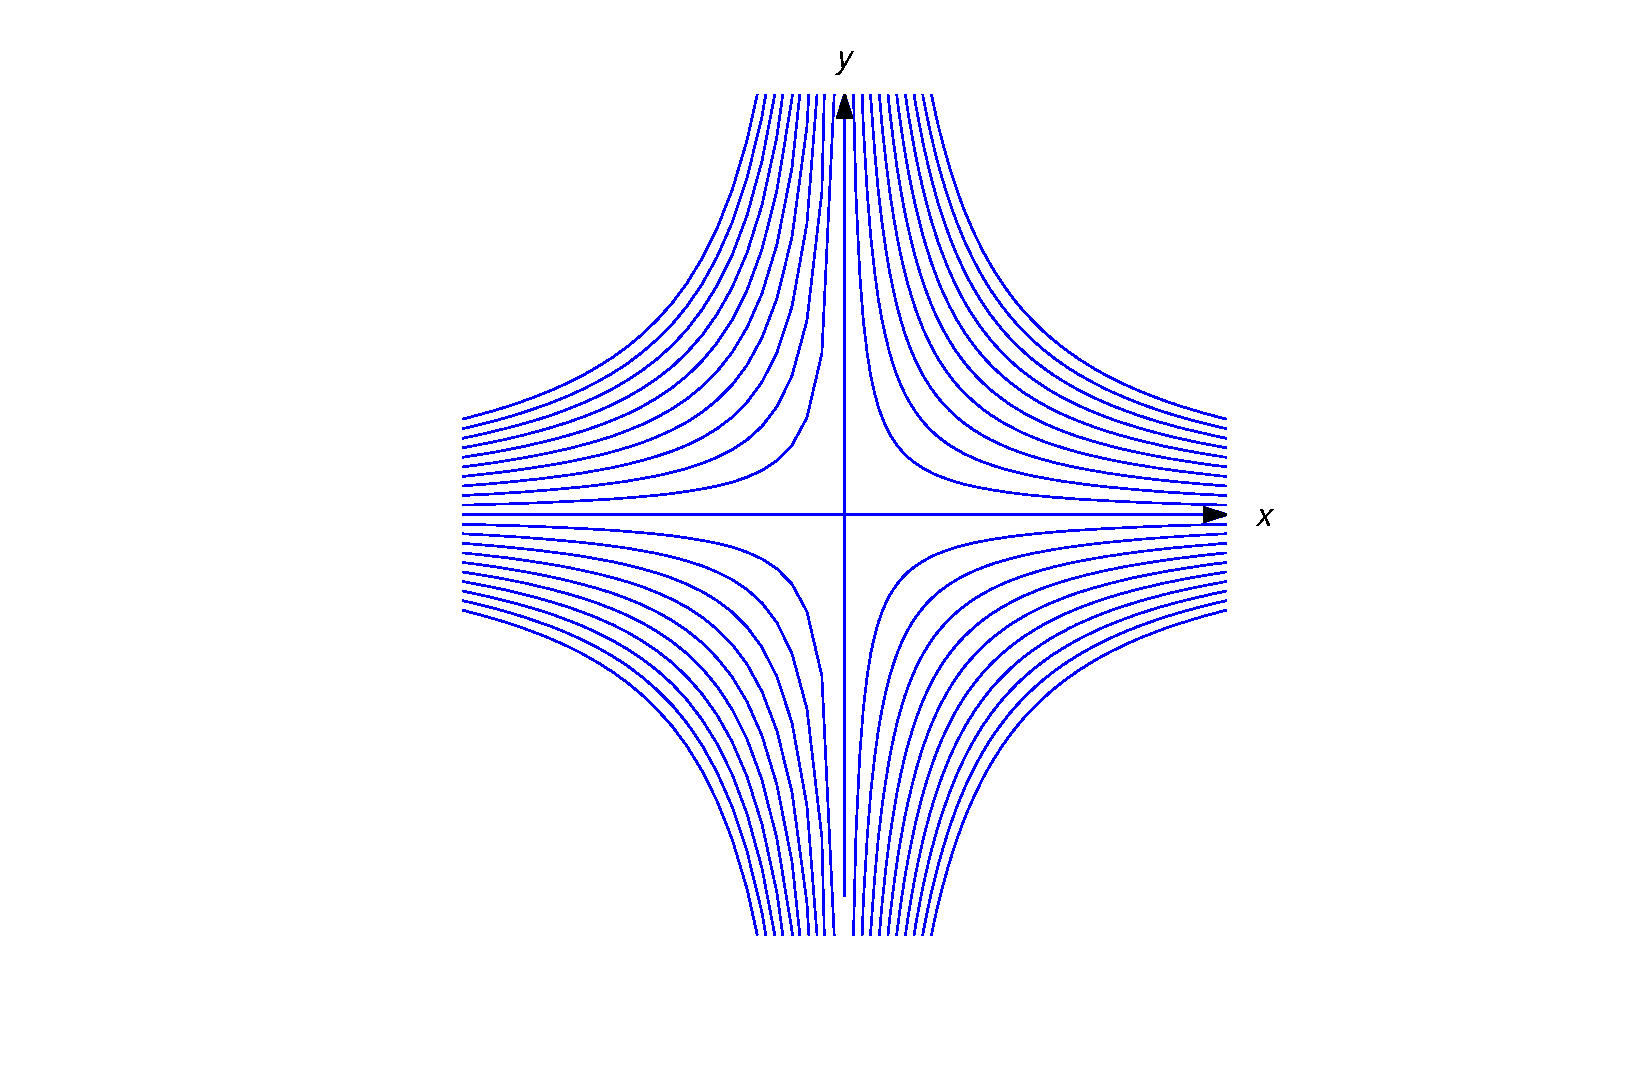
\includegraphics[bb=-78 148 689 643,width=5.67in,height=3.66in,keepaspectratio]{fig040507}}
\caption{}
  \label{figure:4.5.7}
  \end{minipage}
\end{figure}

\begin{example}\label{example:4.5.8}\rm
Find curves $y=y(x)$ such that the tangent line to the curve at any
point $(x_0,y(x_0))$ intersects the $x$-axis at $(x^2_0,0)$.
Figure~\ref{figure:4.5.8} illustrates the situation in the case where
the curve is in the first quadrant and $0<x<1$.
\end{example}

\begin{figure}[htbp]
\color{blue}
  \begin{minipage}[b]{0.5\linewidth}
    \centering
   \scalebox{.65}{
  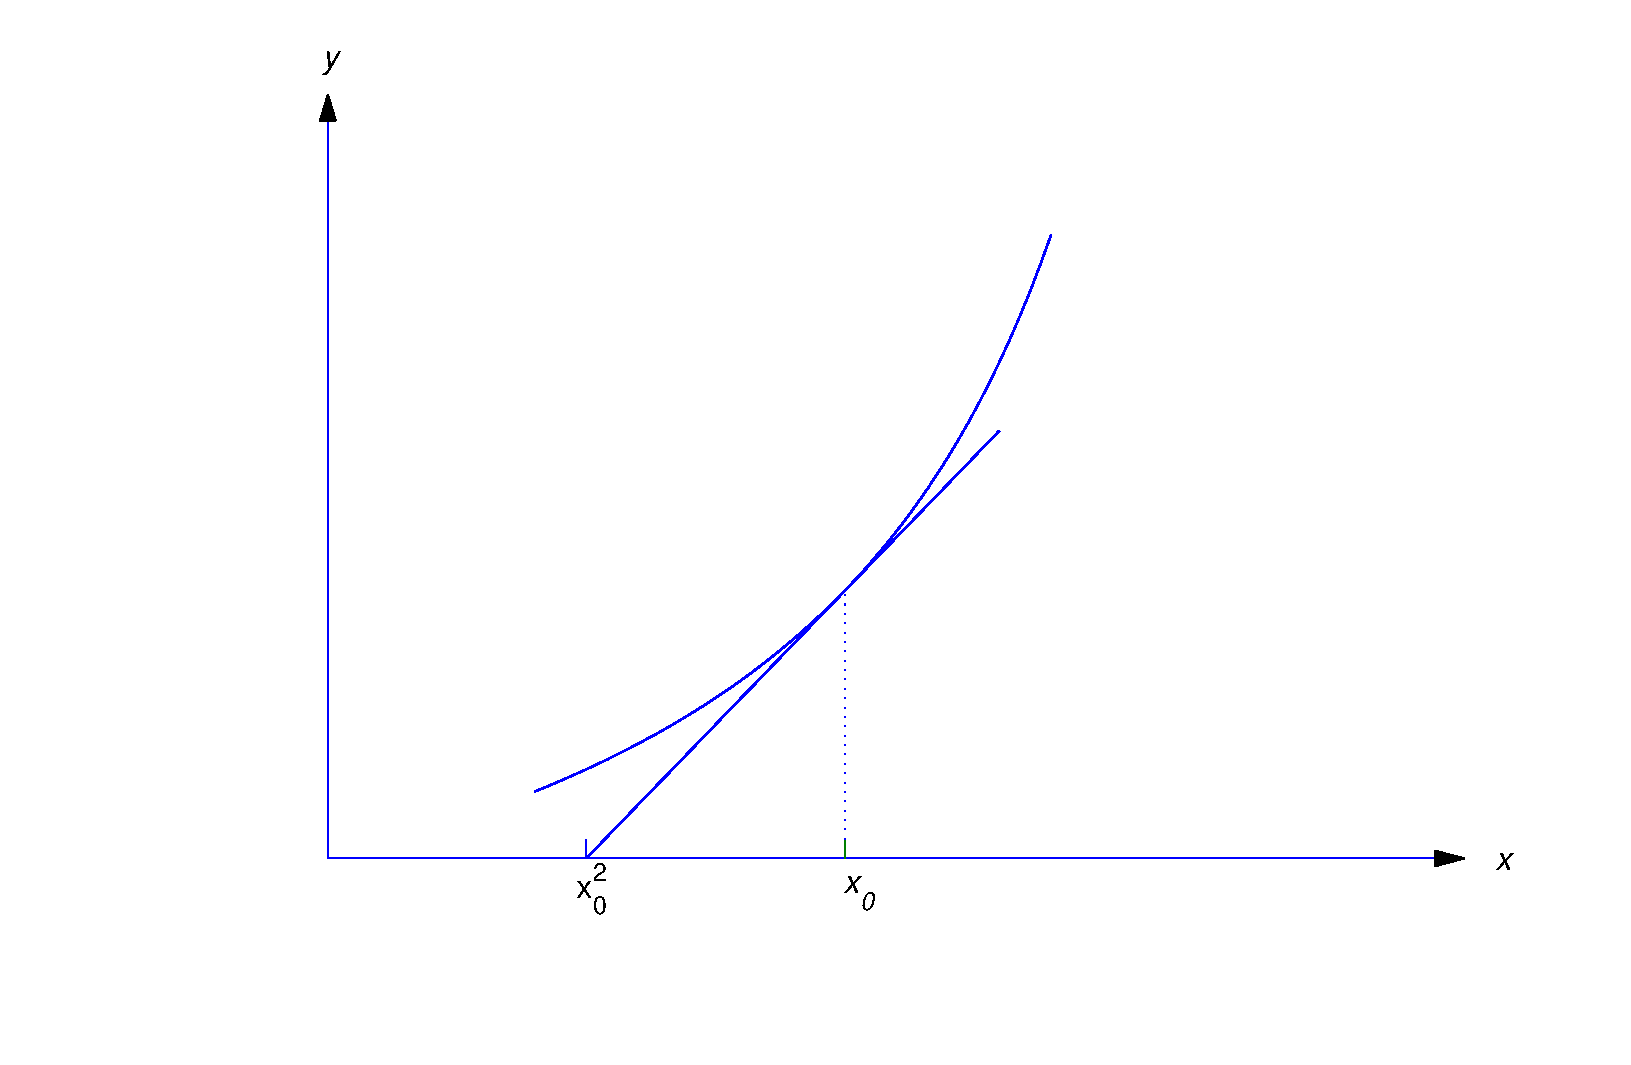
\includegraphics[bb=-78 148 689 643,width=5.67in,height=3.66in,keepaspectratio]{fig040508} }
\caption{}
  \label{figure:4.5.8}
  \end{minipage}
  \hspace{0.6cm}
  \begin{minipage}[b]{0.5\linewidth}
    \centering
   \scalebox{.65}{
  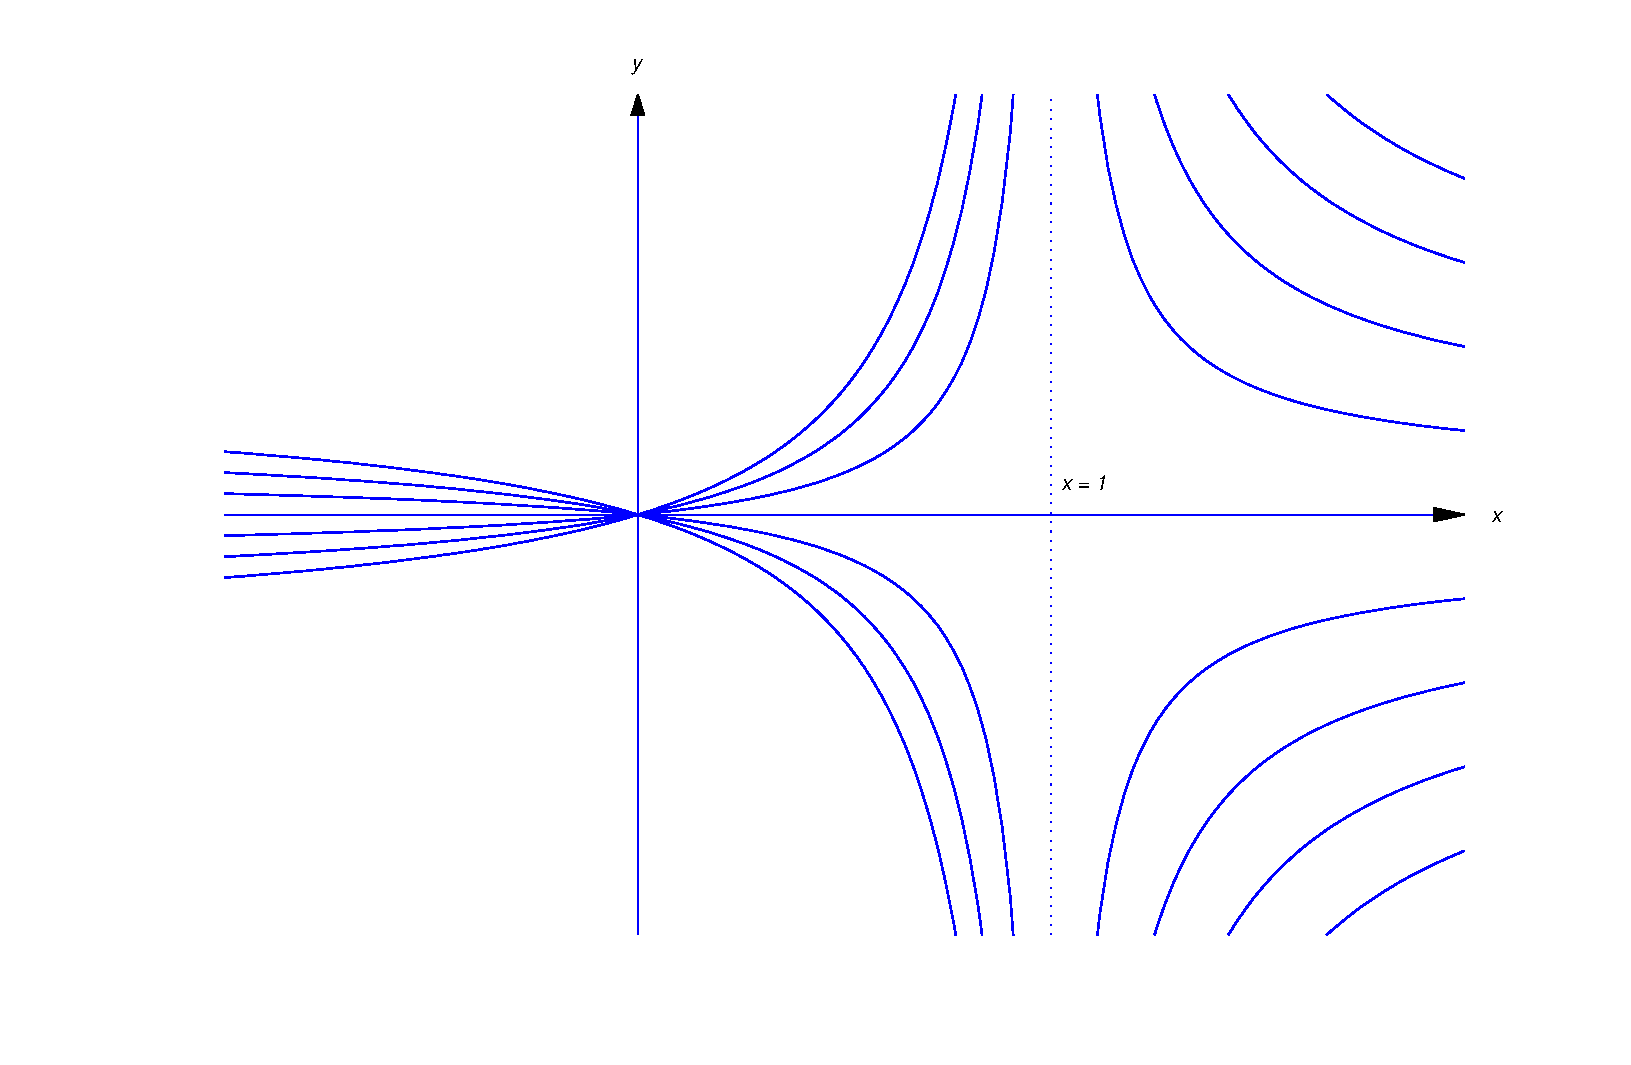
\includegraphics[bb=-78 148 689 643,width=5.67in,height=3.66in,keepaspectratio]{fig040509} }
\caption{}
  \label{figure:4.5.9}
  \end{minipage}
\end{figure}

\solution
The equation of the line tangent to the curve at $(x_0,y(x_0))$ is
$$
y=y(x_0)+y'(x_0)(x-x_0).
$$
Since $(x^2_0,0)$ is on the tangent line,
$$
0=y(x_0)+y'(x_0)(x^2_0-x_0).
$$
Since $x_0$ is arbitrary we drop the subscript and conclude that
$y=y(x)$ satisfies
$$
y+y'(x^2-x)=0.
$$
Therefore
$$
{y'\over y}=-{1\over x^2-x}=-{1\over x(x-1)}={1\over x}-{1\over x-1},
$$
so
$$
\ln|y|=\ln|x|-\ln|x-1|+k=
\ln\left|{x\over x-1}\right|+k,
$$
and
$$
y={cx\over x-1}.
$$
If $c=0$, the graph of this function is the $x$-axis.   If $c\ne0$, it's
a hyperbola with vertical asymptote $x=1$ and horizontal asymptote
$y=c$. Figure~\ref{figure:4.5.9} shows the graphs for $c\ne0$.

\boxit{Orthogonal Trajectories}

\noindent
Two curves $C_1$ and $C_2$ are said to be \it orthogonal \rm at a
point of intersection $(x_0,y_0)$ if they have perpendicular tangents
at $(x_0,y_0)$. (Figure~\ref{figure:4.5.10}). A curve is said to be an
{\color{blue}\it orthogonal trajectory \/} of a given family of curves if it's
orthogonal to every curve in the family. For example, every line
through the origin is an orthogonal trajectory of the family of
circles centered at the origin.  Conversely,
any such circle is an orthogonal trajectory of the family of lines
through the origin (Figure~\ref{figure:4.5.11}).

\begin{figure}[htbp]
\color{blue}
  \begin{minipage}[b]{0.5\linewidth}
    \centering
   \scalebox{.7}{
  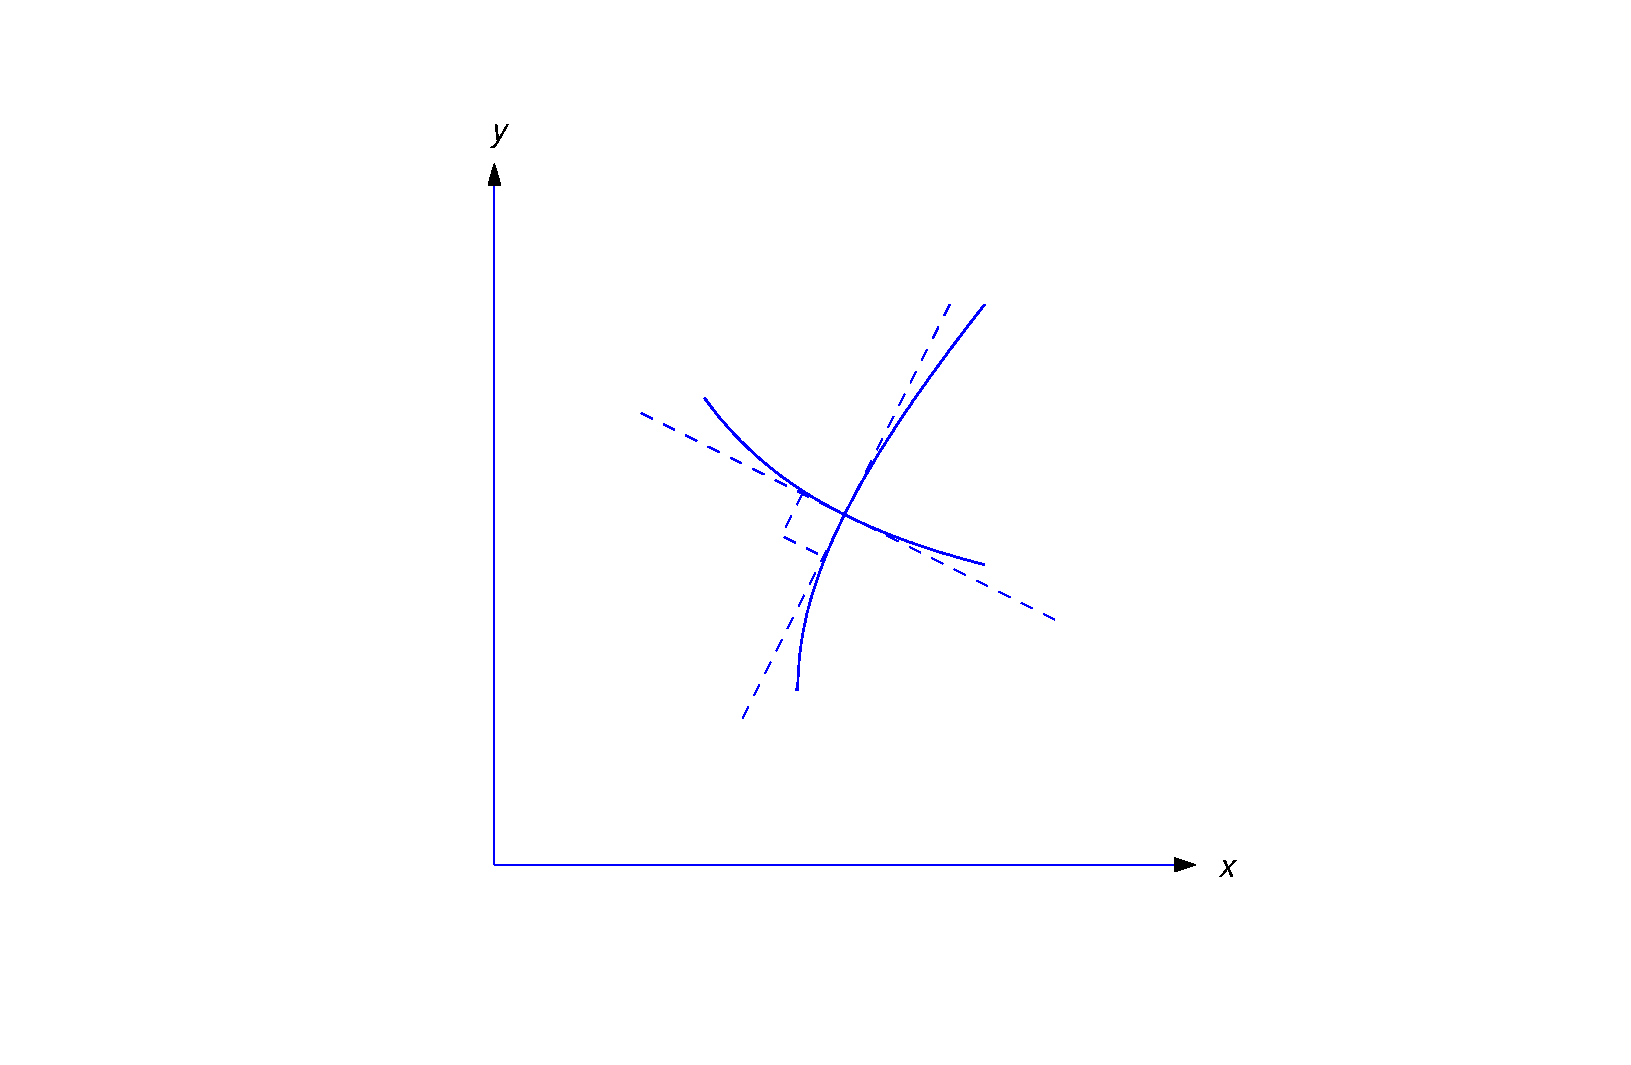
\includegraphics[bb=-78 148 689 643,width=5.67in,height=3.66in,keepaspectratio]{fig040510}}
  \caption{Curves orthogonal at a point of intersection}
  \label{figure:4.5.10}
\end{minipage}
  \begin{minipage}[b]{0.5\linewidth}
    \centering
   \scalebox{.7}{
  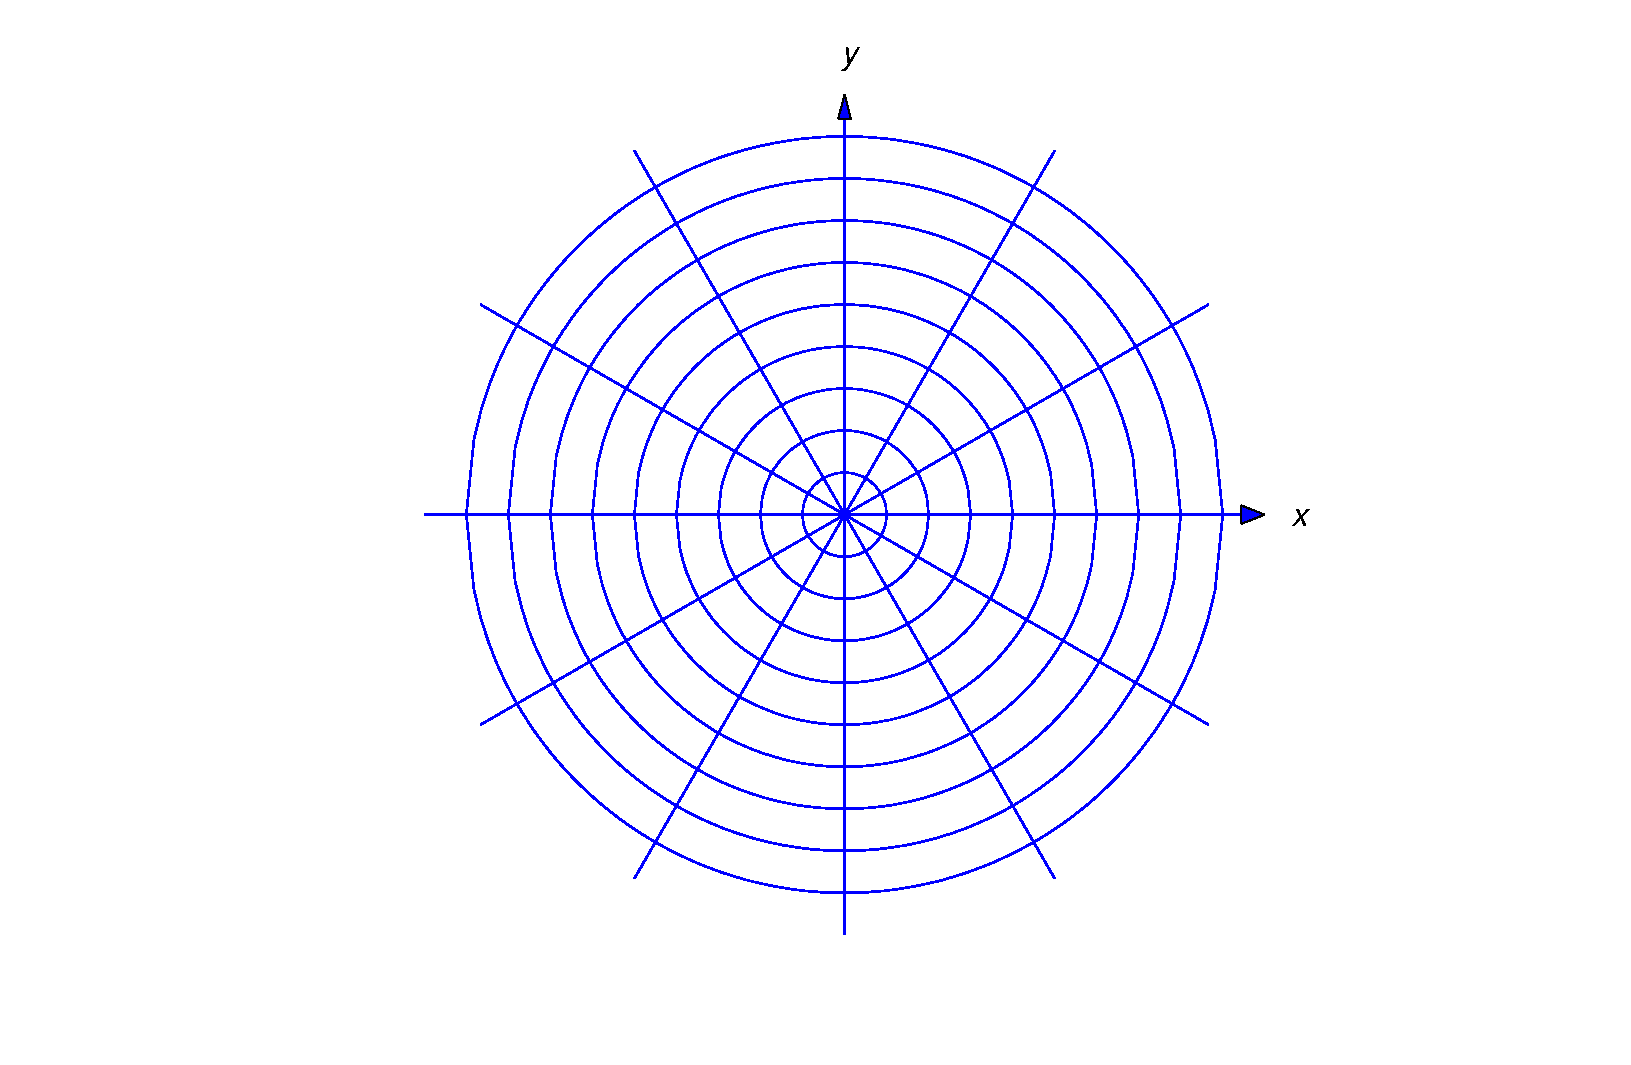
\includegraphics[bb=-78 148 689 643,width=5.67in,height=3.66in,keepaspectratio]{fig040511}}
  \caption{Orthogonal families of circles and lines}
  \label{figure:4.5.11}
\end{minipage}
\end{figure}

Orthogonal trajectories occur in many physical applications.
For example, if $u=u(x,y)$ is the temperature at a point $(x,y)$,  the
curves defined by
\begin{equation} \label{eq:4.5.16}
u(x,y)=c
\end{equation}
are called {\color{blue}\it isothermal\/} curves. The orthogonal trajectories of
this family are called {\color{blue}\it heat-flow\/} lines, because at any given
point the direction of maximum heat flow is perpendicular to the
isothermal through the point. If $u$ represents the potential energy
of an object moving under a force that depends upon $(x,y)$,  the
curves \eqref{eq:4.5.16} are called {\color{blue}\it equipotentials\/}, and the
orthogonal trajectories are called {\color{blue}\it lines of force\/}.

From analytic geometry we know that two nonvertical lines $L_1$ and
$L_2$ with slopes $m_1$ and $m_2$, respectively, are perpendicular if
and only if $m_2=-1/m_1$;  therefore, the integral curves of the
differential equation
$$
y'=-{1\over f(x,y)}
$$
are orthogonal trajectories of the integral curves of the differential
equation
$$
y'=f(x,y),
$$
because at any point $(x_0,y_0)$ where curves from the two families
intersect the slopes of the respective tangent lines are
$$
m_1=f(x_0,y_0)\mbox{\quad and \quad} m_2=-{1\over f(x_0,y_0)}.
$$

This suggests a  method for finding orthogonal trajectories
of a family of integral curves of a first order equation.

\boxit{Finding Orthogonal Trajectories}

{\bf Step 1.} Find a differential equation
$$
y'=f(x,y)
$$
 for the given family.

\medskip

{\bf Step 2.} Solve the differential equation
$$
y'=-{1\over f(x,y)}
$$
to find the orthogonal trajectories.

\begin{example}\label{example:4.5.9} \rm
Find the orthogonal trajectories of the family of circles
\begin{equation} \label{eq:4.5.17}
x^2+y^2=c^2 \quad (c>0).
\end{equation}
\end{example}

\solution
To find a differential equation for the family of circles we
differentiate \eqref{eq:4.5.17} implicitly with respect to $x$ to obtain
$$
2x+2yy'=0,
$$
or
$$
y'=-{x\over y}.
$$
Therefore the integral curves  of
$$
y'={y\over x}
$$
are orthogonal trajectories of the given family. We leave it to you to
verify that the general solution of this equation is
$$
y=kx,
$$
where $k$ is an arbitrary constant. This is the equation of a
nonvertical line through $(0,0)$. The $y$ axis is also an orthogonal
trajectory of the given family. Therefore every line through the
origin is an orthogonal trajectory of the given family \eqref{eq:4.5.17}
(Figure~\ref{figure:4.5.11}). This is consistent with the theorem of plane
geometry which states that a diameter of a circle and a tangent line
to the circle at the end of the diameter are perpendicular.

\begin{example}\label{example:4.5.10} \rm
Find the orthogonal trajectories of the family of hyperbolas
\begin{equation}  \label{eq:4.5.18}
xy=c \quad (c\ne0)
\end{equation}
(Figure~\ref{figure:4.5.7}).
\end{example}

\solution
Differentiating \eqref{eq:4.5.18} implicitly with respect to $x$ yields
$$
y+xy'=0,
$$
or
$$
y'=-{y\over x};
$$
 thus, the integral curves of
$$
y'={x\over y}
$$
are orthogonal trajectories of the given family. Separating variables
yields
$$
y'y=x
$$
and integrating yields
$$
y^2-x^2=k,
$$
which is the equation of a hyperbola if $k \ne0$, or of the lines
$y=x$ and $y=-x$ if $k=0$ (Figure~\ref{figure:4.5.12}).

\begin{figure}[tbp]
  \centering
  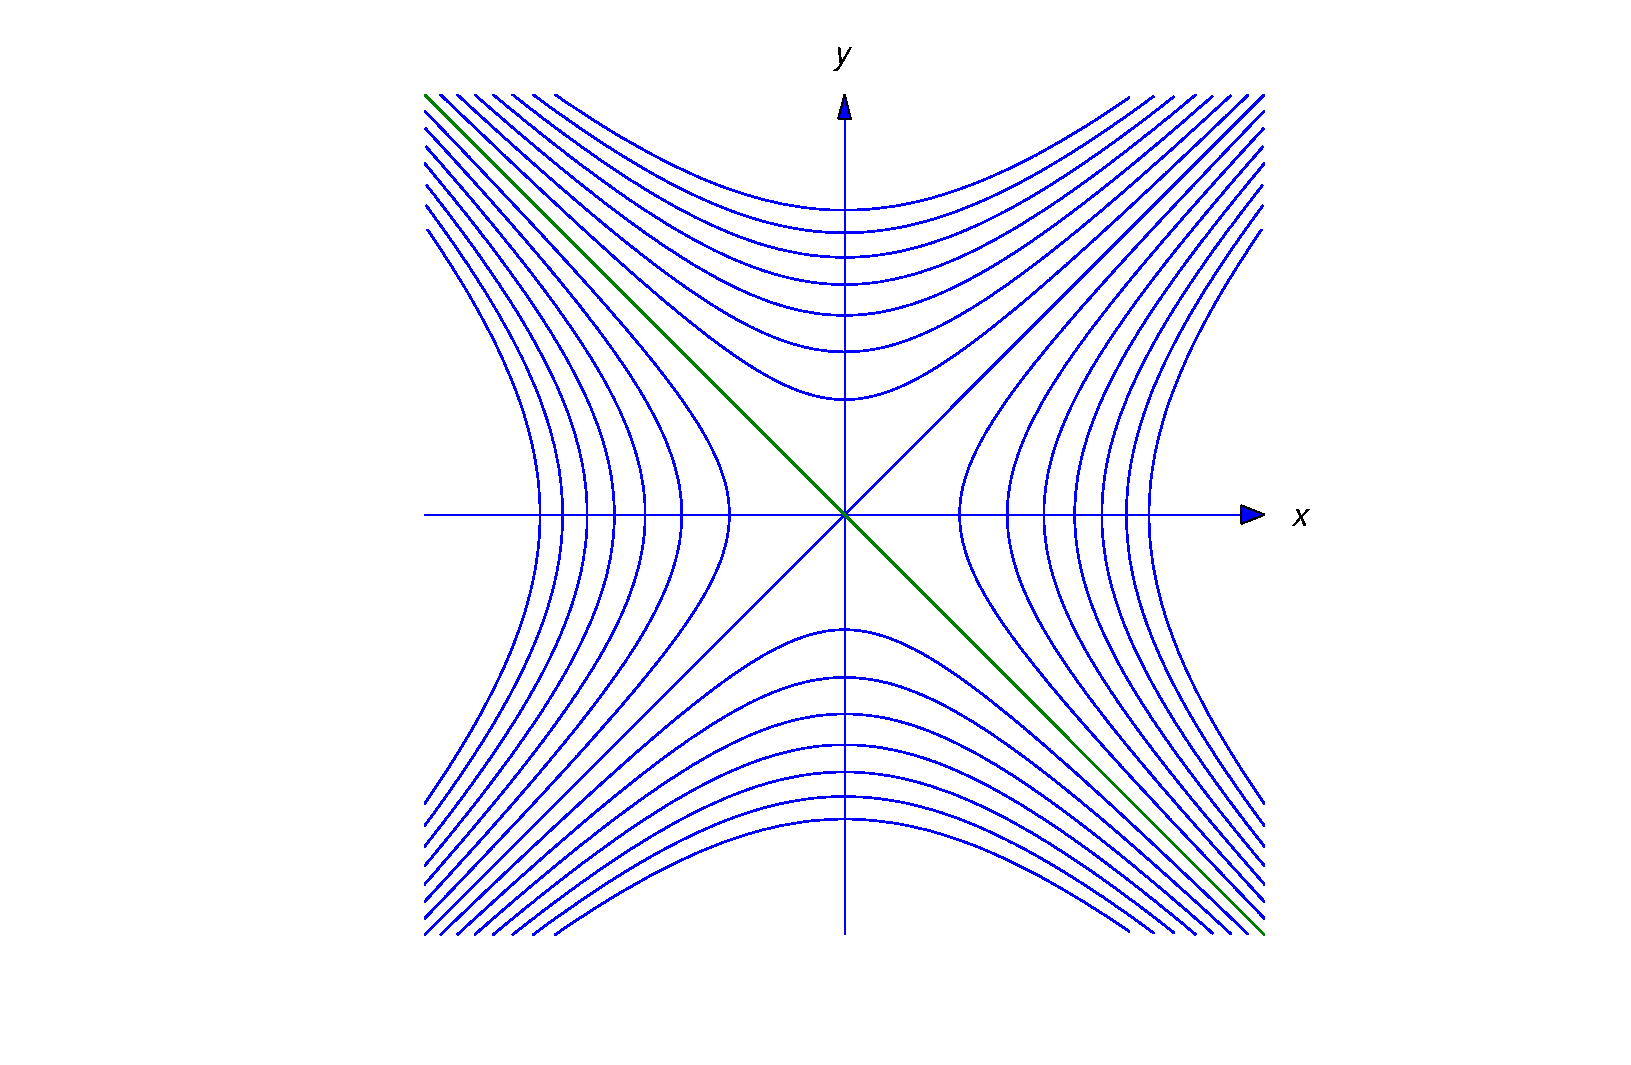
\includegraphics[bb=-78 148 689 643,width=5.67in,height=3.66in,keepaspectratio]{fig040512}
\color{blue}
\caption{ Orthogonal trajectories of the hyperbolas $xy=c$}
  \label{figure:4.5.12}
\end{figure}

\begin{example}\rm
Find the orthogonal trajectories of the family of circles defined by
\begin{equation} \label{eq:4.5.19}
(x-c)^2+y^2=c^2 \quad (c\ne0).
\end{equation}
 These circles are centered on the $x$-axis and tangent to the
$y$-axis (Figure~\ref{figure:4.5.13}\part{a}).
\end{example}

\solution
Multiplying out the left side of \eqref{eq:4.5.19} yields
\begin{equation} \label{eq:4.5.20}
x^2-2cx+y^2=0,
\end{equation}
and differentiating this implicitly with respect to $x$ yields
\begin{equation} \label{eq:4.5.21}
2(x-c)+2yy'=0.
\end{equation}
 From \eqref{eq:4.5.20},
$$
c={x^2+y^2\over2x},
$$
so
$$
x-c=x-{x^2+y^2\over2x}={x^2-y^2\over2x}.
$$
Substituting this into \eqref{eq:4.5.21} and solving for $y'$ yields
\begin{equation} \label{eq:4.5.22}
y'={y^2-x^2\over2xy}.
\end{equation}
The curves defined by \eqref{eq:4.5.19} are integral curves of
\eqref{eq:4.5.22}, and the integral curves of
$$
y'={2xy\over x^2-y^2}
$$
are orthogonal trajectories of the family \eqref{eq:4.5.19}. This is a
homogeneous nonlinear equation, which we studied in
Section~2.4. Substituting $y=ux$ yields
$$
u'x+u={2x(ux)\over x^2-(ux)^2}={2u\over1-u^2},
$$
so
$$
u'x={2u\over1-u^2}-u={u(u^2+1)\over1-u^2},
$$
Separating variables yields
$$
{1-u^2\over u(u^2+1)}u'={1\over x},
$$
or, equivalently,
$$
\left[{1\over u}-{2u\over u^2+1}\right]u'={1\over x}.
$$
Therefore
$$
\ln |u|-\ln (u^2+1)=\ln |x|+k.
$$
By substituting $u=y/x$, we see that
$$
\ln|y|-\ln|x|-\ln(x^2+y^2)+\ln(x^2)=\ln|x|+k,
$$
which, since $\ln(x^2)=2\ln|x|$, is equivalent to
$$
\ln|y|-\ln(x^2+y^2)=k,
$$
or
$$
|y|=e^k(x^2+y^2).
$$
To see what these curves are we rewrite this equation as
$$
x^2+|y|^2-e^{-k}|y|=0
$$
and complete the square to obtain
$$
x^2+(|y|-e^{-k}/2)^2=(e^{-k}/2)^2.
$$
This can be rewritten as
$$
x^2+(y-h)^2=h^2,
$$
where
$$
h=\left\{\begin{array}{rl} \dst{e^{-k}\over2}&\mbox{ if } y\ge
0,\\[\jot]-\dst{e^{-k}\over2}&\mbox{ if } y\le0. \end{array}\right.
$$
Thus, the orthogonal trajectories are circles centered on the $y$ axis
and tangent to the $x$ axis (Figure~\ref{figure:4.5.13}(b)). The circles
for which $h>0$ are above the $x$-axis, while those for which $h<0$
are below.

\enlargethispage{2in}

\begin{figure}[H]
  \centering
\scalebox{.9}{
  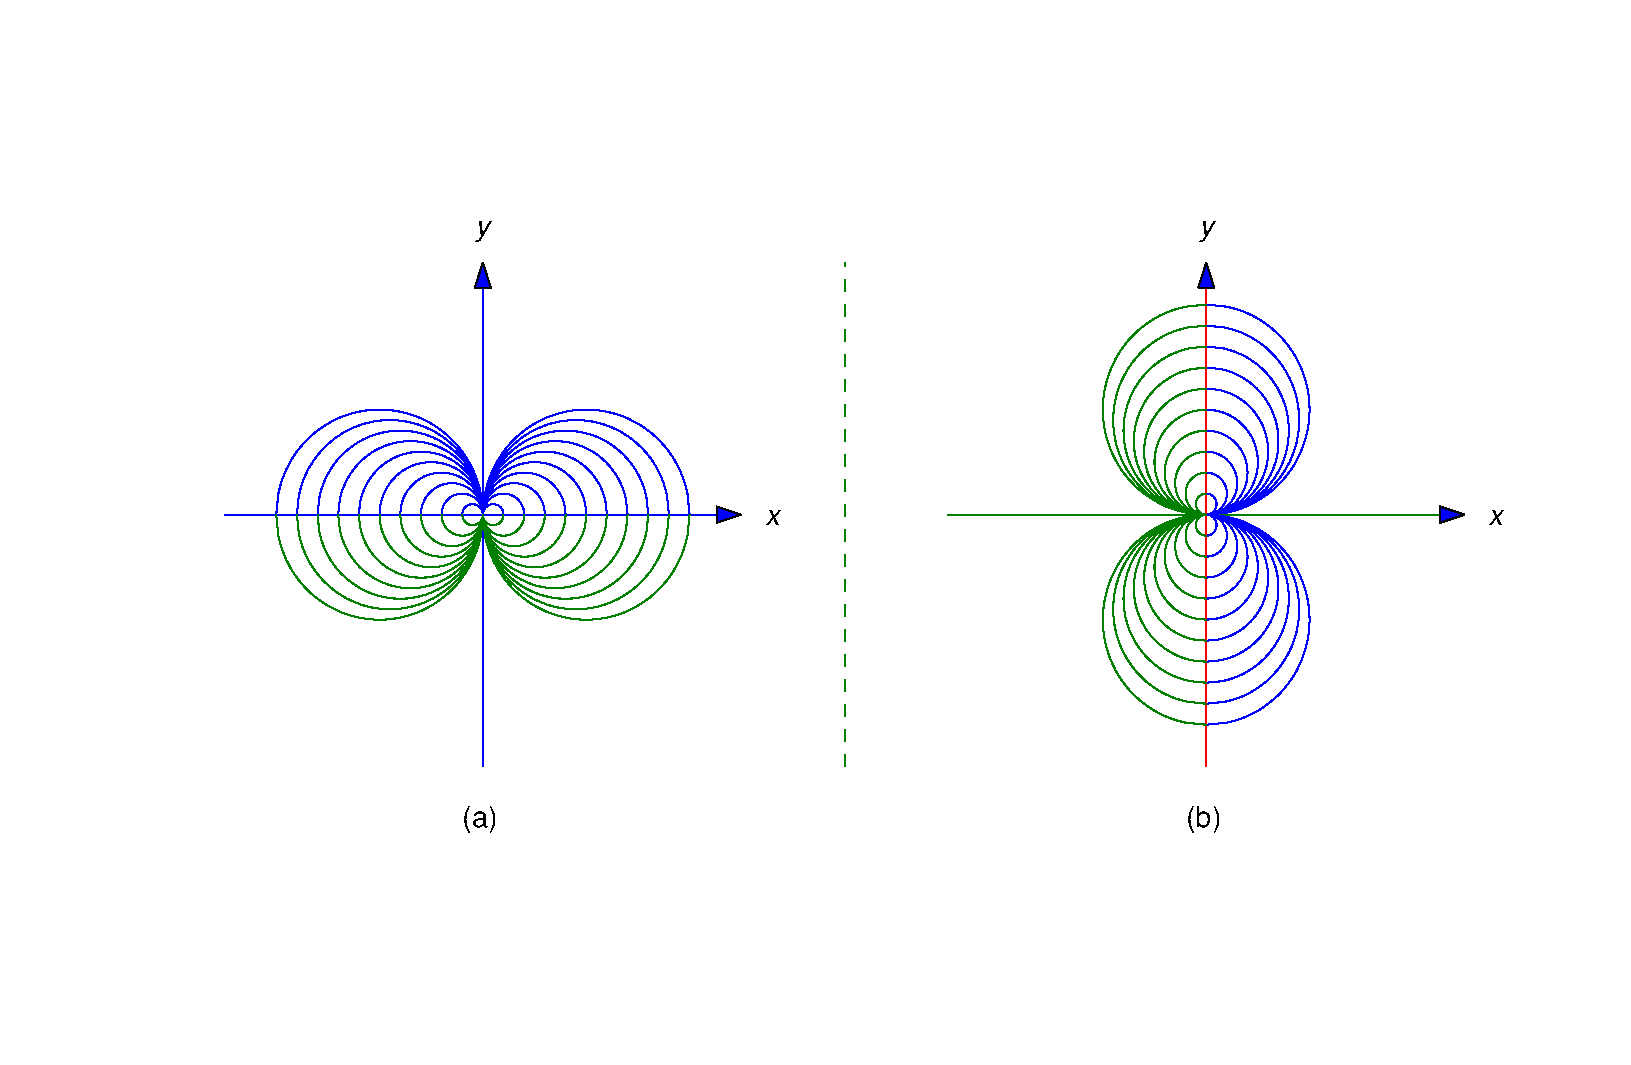
\includegraphics[bb=-78 148 689 643,width=5.67in,height=3.66in,keepaspectratio]{fig040513}}
\color{blue}
\caption{{\bf (a)} The circles $(x-c)^2+y^2=c^2$ \, {\bf (b)} The circles
$x^2+(y-h)^2=h^2$}
\vspace*{-40pt}
  \label{figure:4.5.13}
\end{figure}

\newpage

\exercises
In  Exercises \ref{exer:4.5.1}--\ref{exer:4.5.8} find a first order
differential equation for the given family of curves.

\begin{exerciselist}

\begin{tabular}[t]{@{}p{168pt}@{}p{168pt}}
\item\label{exer:4.5.1} $y(x^2+y^2)=c$
&\vspace*{10pt}\item\label{exer:4.5.2} $e^{xy}=cy$
\end{tabular}

\begin{tabular}[t]{@{}p{168pt}@{}p{168pt}}
 \item\label{exer:4.5.3} $\ln |xy|=c(x^2+y^2)$&
 \item\label{exer:4.5.4} $y=x^{1/2}+cx$
\end{tabular}

\begin{tabular}[t]{@{}p{168pt}@{}p{168pt}}
\item\label{exer:4.5.5} $y=e^{x^2}+ce^{-x^2}$&
 \item\label{exer:4.5.6} $\dst{y=x^3+{c\over x}}$
\end{tabular}

\begin{tabular}[t]{@{}p{168pt}@{}p{168pt}}
\item\label{exer:4.5.7} $y=\sin x+ce^x$&
\item\label{exer:4.5.8} $y=e^x+c(1+x^2)$
\end{tabular}

\item\label{exer:4.5.9}
Show that the family of circles
$$
(x-x_0)^2+y^2=1,\;-\infty<x_0<\infty,
$$
can be obtained by joining integral curves of two first order
differential equations. More specifically, find differential equations
for the families of semicircles
$$
(x-x_0)^2+y^2=1,\; x_0<x<x_0+1,\;-\infty<x_0<\infty,
$$
$$
(x-x_0)^2+y^2=1,\; x_0-1<x<x_0,\;-\infty<x_0<\infty.
$$

\item\label{exer:4.5.10}
Suppose $f$ and $g$ are differentiable for all $x$. Find a
differential equation for the family of functions $y=f+cg$
($c$=constant).

\exercisetext{In Exercises \ref{exer:4.5.11}--\ref{exer:4.5.13} find a
first order differential equation for the given family of curves.}

\item\label{exer:4.5.11}
Lines through a given point $(x_0,y_0)$.

\item\label{exer:4.5.12}
Circles through $(-1,0)$ and $(1,0)$.

\item\label{exer:4.5.13}
Circles through $(0,0)$ and $(0,2)$.

\item\label{exer:4.5.14}
Use the method Example~\ref{example:4.5.6}{\bf (a)} to find the equations
of lines through the given points tangent to the parabola $y=x^2$.
Also, find the points of tangency.

\begin{tabular}[t]{@{}p{78pt}@{}p{78pt}p{78pt}p{78pt}}
{\bf (a)}\; $(5,9)$
&{\bf (b)}\; $(6,11)$
&{\bf (c)}\; $(-6,20)$
&{\bf (d)}\; $(-3,5)$
\end{tabular}

\item\label{exer:4.5.15}
\begin{alist}
\item % (a)
Show that the equation of the line tangent to the circle
$$
x^2+y^2=1
\eqno{\rm (A)}
$$
at a point $(x_0,y_0)$  on the circle is
$$
y=\dst{1-x_0x\over y_0}\mbox{\quad if \quad} x_0\ne\pm1.
\eqno{\rm (B)}
$$
\item % (b)
Show that if $y'$ is the slope of a nonvertical tangent line to the
circle (A) and $(x,y)$ is a point on the tangent line then
$$
(y')^2(x^2-1)-2xyy'+y^2-1=0.
\eqno{\rm (C)}
$$
\item % (c)
Show that the segment of the tangent line (B) on which $(x-x_0)/y_0>0$
is an integral curve of the differential equation
$$
y'={xy-\sqrt{x^2+y^2-1}\over x^2-1},
\eqno{\rm (D)}
$$
while the segment on which $(x-x_0)/y_0<0$ is an integral curve of the
differential equation
$$
y'={xy+\sqrt{x^2+y^2-1}\over x^2-1}.
\eqno{\rm (E)}
$$

\hint{Use the quadratic formula to solve ${\rm (C)}$ for
$y'$. Then substitute {\rm (B)} for $y$ and
 choose the $\pm$ sign in the quadratic formula so that the
resulting expression for $y'$ reduces to the known slope
$y'=-x_0/y_0$.}

\item % (d)
Show that the upper and lower semicircles of (A) are also integral
curves of (D) and (E).

\item % (e)
Find the equations of two lines through (5,5) tangent to the circle
(A), and find the points of tangency.
\end{alist}

\item\label{exer:4.5.16}
\begin{alist}
\item % (a)
Show that the equation of the line tangent to the  parabola
$$
x=y^2
\eqno{\rm (A)}
$$
at a point $(x_0,y_0)\ne(0,0)$  on the parabola is
$$
y=\dst{y_0\over2}+\dst{x\over2y_0}.
\eqno{\rm (B)}
$$
\item % (b)
Show that if $y'$ is the slope of a nonvertical tangent line
to the parabola (A) and $(x,y)$ is a point on the tangent
line then
$$
4x^2(y')^2-4xyy'+x=0.
\eqno{\rm (C)}
$$
\item % (c)
Show that the segment of the tangent line defined in \part{a} on which
$x>x_0$ is an integral curve of the differential equation
$$
y'={y+\sqrt{y^2-x}\over2x},
\eqno{\rm (D)}
$$
while the segment on which $x<x_0$ is an integral curve of the
differential equation
$$
y'={y-\sqrt{y^2-x}\over2x},
\eqno{\rm (E)}
$$

\hint{Use the quadratic formula to solve ${\rm (C)}$ for $y'$. Then
substitute {\rm (B)} for $y$ and choose the $\pm$ sign in the
quadratic formula so that the resulting expression for $y'$ reduces to
the known slope $y'=\dst{1\over2y_0}$.}

\item % (d)
Show that the upper and lower halves of the parabola (A), given by
$y=\sqrt x$ and $y=-\sqrt x$ for $x>0$, are also integral curves of
(D) and (E).
\end{alist}

\item\label{exer:4.5.17}
Use the results of Exercise \ref{exer:4.5.16} to find the equations of two
lines tangent to the parabola $x=y^2$ and passing through the given
point. Also find the points of tangency.

\begin{tabular}[t]{@{}p{78pt}@{}p{78pt}p{78pt}p{78pt}}
{\bf (a)}\; $(-5,2)$
&{\bf (b)}\; $(-4,0)$
&{\bf (c)}\; $(7,4)$
&{\bf (d)}\; $(5,-3)$
\end{tabular}

\item\label{exer:4.5.18}
Find a curve $y=y(x)$ through (1,2) such that the tangent to the curve
at any point $(x_0,y(x_0))$ intersects the $x$ axis at
$\dst{x_I=x_0/2}$.

\item\label{exer:4.5.19}
Find all curves $y=y(x)$ such that the tangent to the curve at any
point $(x_0,y(x_0))$ intersects the $x$ axis at $x_I=x^3_0$.

\item\label{exer:4.5.20}
Find all curves $y=y(x)$ such that the tangent to the curve at any
point passes through a given point $(x_1,y_1)$.

\item\label{exer:4.5.21}
Find a curve $y=y(x)$ through $(1,-1)$ such that the tangent to the
curve at any point $(x_0,y(x_0))$ intersects the $y$ axis at
$y_I=x^3_0$.

\item\label{exer:4.5.22}
Find all curves $y=y(x)$ such that the tangent to the curve at any
point $(x_0,y(x_0))$ intersects the $y$ axis at $y_I=x_0$.

\item\label{exer:4.5.23}
Find a curve $y=y(x)$ through $(0,2)$ such that the normal to the
curve at any point $(x_0,y(x_0))$ intersects the $x$ axis at
$x_I=x_0+1$.

\item\label{exer:4.5.24}
Find a curve $y=y(x)$ through $(2,1)$ such that the normal to the
curve at any point $(x_0,y(x_0))$ intersects the $y$ axis at
$y_I=2y(x_0)$.

\exercisetext{In Exercises \ref{exer:4.5.25}--\ref{exer:4.5.29} find the
orthogonal trajectories of the given family of curves.}

\begin{tabular}[t]{@{}p{168pt}@{}p{168pt}}
\item\label{exer:4.5.25} $x^2+2y^2=c^2$
&\vspace*{10pt}\item\label{exer:4.5.26} $x^2+4xy+y^2=c$
\end{tabular}

\begin{tabular}[t]{@{}p{168pt}@{}p{168pt}}
\item\label{exer:4.5.27} $y=ce^{2x}$
&\item\label{exer:4.5.28} $xye^{x^2}=c$
\end{tabular}

\item\label{exer:4.5.29}
$\dst{y={ce^x\over x}}$

\item\label{exer:4.5.30}
Find a curve through $(-1,3)$ orthogonal to every parabola of the form
$$
y=1+cx^2
$$
that it intersects. Which of these parabolas does the desired curve
intersect?

\item\label{exer:4.5.31}
Show that the orthogonal trajectories of
$$
x^2+2axy+y^2=c
$$
satisfy
$$
|y-x|^{a+1}|y+x|^{a-1}=k.
$$

\item\label{exer:4.5.32}
If lines $L$ and $L_1$ intersect at $(x_0,y_0)$ and $\alpha$ is the
smallest angle through which $L$ must be rotated counterclockwise
about $(x_0,y_0)$ to bring it into coincidence with $L_1$, we say that
$\alpha$ is the {\color{blue}\it angle from $L$ to $L_1$\/};   thus,
$0\le\alpha<\pi$. If $L$ and $L_1$ are tangents to curves $C$ and
$C_1$, respectively, that intersect at $(x_0,y_0)$, we say that $C_1$
intersects $C$ at the angle $\alpha$. Use the identity
$$
\tan(A+B)={\tan A+\tan B\over1-\tan A\tan B}
$$
to show that if $C$ and $C_1$ are intersecting integral curves of
$$
y'=f(x,y)  \mbox{\quad and \quad} y'={f(x,y)+\tan\alpha\over
1-f(x,y)\tan\alpha} \quad\left( \alpha \ne {\pi\over2}\right),
$$
respectively, then $C_1$ intersects $C$ at the angle $\alpha$.

\item\label{exer:4.5.33}
Use the result of Exercise~\ref{exer:4.5.32} to find a family of curves
that intersect every nonvertical line through the origin at the angle
$\alpha=\pi/4$.

\item\label{exer:4.5.34}
Use the result of Exercise~\ref{exer:4.5.32} to find a family of curves
that intersect every circle centered at the origin at a given angle
$\alpha \ne \pi/2$.

\end{exerciselist}

